\documentclass[12pt, a4paper, oneside]{report}

% ── Packages ──────────────────────────────────────────────────────────────────
\usepackage[a4paper, top=1in, bottom=1in, left=1.25in, right=1in]{geometry}
\usepackage{fontenc}
\usepackage{inputenc}
\usepackage{setspace}
\usepackage{parskip}
\usepackage{titlesec}
\usepackage{fancyhdr}
\usepackage{graphicx}
\usepackage{booktabs}
\usepackage{array}
\usepackage{tabularx}
\usepackage{longtable}
\usepackage{multirow}
\usepackage{xcolor}
\usepackage{colortbl}
\usepackage{amsmath}
\usepackage{amssymb}
\usepackage{hyperref}
\usepackage{caption}
\usepackage{subcaption}
\usepackage{enumitem}
\usepackage{natbib}
\usepackage{microtype}
\usepackage{float}
\usepackage{listings}
\usepackage{tocloft}
\usepackage{emptypage}

% ── Colours ───────────────────────────────────────────────────────────────────
\definecolor{headerblue}{RGB}{31, 73, 125}
\definecolor{rowshade}{RGB}{235, 245, 251}
\definecolor{bestrow}{RGB}{213, 245, 227}
\definecolor{deeprow}{RGB}{232, 248, 245}
\definecolor{linkblue}{RGB}{0, 90, 160}

% ── Hyperref setup ────────────────────────────────────────────────────────────
\hypersetup{
    colorlinks=true,
    linkcolor=linkblue,
    citecolor=linkblue,
    urlcolor=linkblue,
    pdftitle={Detection of AI-Generated and Cloned Speech for Banking Voice Authentication},
    pdfauthor={Rajib Roy},
}

% ── Typography ────────────────────────────────────────────────────────────────
\onehalfspacing
\setlength{\parindent}{0pt}
\setlength{\parskip}{8pt}

% ── Chapter/section titles ────────────────────────────────────────────────────
\titleformat{\chapter}[display]
  {\normalfont\Large\bfseries\color{headerblue}}
  {\chaptertitlename\ \thechapter}{12pt}{\Huge}
\titlespacing*{\chapter}{0pt}{-10pt}{20pt}

\titleformat{\section}
  {\normalfont\large\bfseries\color{headerblue}}
  {\thesection}{1em}{}
\titlespacing*{\section}{0pt}{16pt}{6pt}

\titleformat{\subsection}
  {\normalfont\normalsize\bfseries}
  {\thesubsection}{1em}{}
\titlespacing*{\subsection}{0pt}{12pt}{4pt}

% ── Header / footer ───────────────────────────────────────────────────────────
\pagestyle{fancy}
\fancyhf{}
\fancyhead[L]{\small\textit{Detection of AI-Generated Speech for Banking Authentication}}
\fancyhead[R]{\small\textit{Rajib Roy | 24459}}
\fancyfoot[C]{\thepage}
\renewcommand{\headrulewidth}{0.4pt}

% ── Caption style ─────────────────────────────────────────────────────────────
\captionsetup{font=small, labelfont=bf, skip=6pt}

% ── Table helpers ─────────────────────────────────────────────────────────────
\newcolumntype{L}[1]{>{\raggedright\arraybackslash}p{#1}}
\newcolumntype{C}[1]{>{\centering\arraybackslash}p{#1}}
\newcolumntype{R}[1]{>{\raggedleft\arraybackslash}p{#1}}

\newcommand{\tblhead}[1]{\cellcolor{headerblue}\textcolor{white}{\textbf{#1}}}
\newcommand{\rowA}{\rowcolor{white}}
\newcommand{\rowB}{\rowcolor{gray!8}}
\newcommand{\rowbest}{\rowcolor{bestrow}}
\newcommand{\rowdeep}{\rowcolor{deeprow}}

% ─────────────────────────────────────────────────────────────────────────────
\begin{document}

% ══════════════════════════════════════════════════════════════════════════════
% TITLE PAGE
% ══════════════════════════════════════════════════════════════════════════════
\begin{titlepage}
\begin{center}
\vspace*{1cm}

{\large M.Tech.\ (Online) --- Artificial Intelligence}\\[4pt]
{\large Indian Institute of Science, Bangalore}\\[2cm]

{\Huge\bfseries\color{headerblue} PROJECT REPORT}\\[1.1cm]

{\LARGE\bfseries Detection of AI-Generated and Cloned Speech\\[6pt]
to Strengthen Voice-Based Authentication\\[6pt]
in Banking Environments}\\[2.5cm]

{\large Submitted by}\\[8pt]
{\Large\bfseries Rajib Roy}\\[6pt]
{\large Student Number: 24459}\\[3cm]

{\large Submitted in partial fulfilment of the requirements for the degree of}\\[8pt]
{\large\bfseries Master of Technology in Artificial Intelligence}\\[3cm]

{\large August 2026}

\end{center}
\end{titlepage}

% ══════════════════════════════════════════════════════════════════════════════
% ABSTRACT
% ══════════════════════════════════════════════════════════════════════════════
\chapter*{Abstract}
\addcontentsline{toc}{chapter}{Abstract}

Voice-based authentication is widely used in banking and financial services for transaction approvals and customer verification. Recent advances in neural text-to-speech (TTS) synthesis and voice cloning have created a serious security threat: adversaries can generate highly convincing synthetic speech from a few seconds of a target's voice, enabling impersonation attacks that bypass voice biometric systems. This project addresses the automatic detection of AI-generated and cloned speech under real-world banking telephony conditions.

A comprehensive detection framework was developed and validated using 17,947 audio utterances drawn from 10 distinct sources --- including LibriSpeech genuine speech and synthetic speech from ASVspoof 2019 (six TTS/voice-conversion systems), VITS, Tacotron2, and Microsoft Edge-TTS. All audio was processed at 8\,kHz with G.711 codec simulation to replicate banking channel conditions, with utterances trimmed to 3--8 seconds to match typical transaction confirmation phrases.

Five classification systems were evaluated: SVM, Random Forest, and Gradient Boosting trained on 257-dimensional handcrafted acoustic feature vectors, and two deep learning models --- a CNN and a CNN-LSTM --- trained on 128-bin log-Mel spectrograms. The CNN-LSTM achieved the best performance with an Equal Error Rate (EER) of 0.0035 and F1 of 0.9965 on the standard test set, and a near-perfect EER of 0.0004 on a held-out generalization test comprising Microsoft Edge-TTS --- a TTS system unseen during training. The SVM baseline achieved EER of 0.0083 using only handcrafted features, demonstrating that carefully engineered spectral features are highly discriminative even without deep learning.

Feature analysis revealed that MFCC delta coefficients (encoding temporal rate-of-change) and spectral shape features are the strongest discriminators between genuine and synthetic speech. Robustness evaluation under additive noise (5--20\,dB SNR) and G.711 compression showed that Gradient Boosting is the most noise-robust classical model. The strong cross-system generalization results suggest that spectral artifacts are a common property of neural TTS architectures regardless of the specific system, supporting deployment in banking environments where the attacking TTS system is unknown.

\bigskip
\noindent\textbf{Keywords:} AI-generated speech detection, anti-spoofing, voice biometrics, banking security, TTS detection, MFCC, CNN-LSTM, ASVspoof, telephony authentication

% ══════════════════════════════════════════════════════════════════════════════
% TABLE OF CONTENTS
% ══════════════════════════════════════════════════════════════════════════════
\tableofcontents
\listoffigures
\listoftables
\newpage

% ══════════════════════════════════════════════════════════════════════════════
% CHAPTER 1: INTRODUCTION
% ══════════════════════════════════════════════════════════════════════════════
\chapter{Introduction}

\section{Background and Motivation}

Voice-based authentication has become a standard component of customer verification workflows in banks, call centres, and digital financial platforms. Its appeal is intuitive: a customer's voice is unique, always available, and requires no additional hardware. Transaction confirmations, account access, and high-value transfers are routinely authorized through spoken phrases in automated interactive voice response (IVR) systems and live agent calls.

However, the same years that saw voice authentication proliferate also witnessed a transformation in synthetic speech technology. Neural TTS systems --- beginning with WaveNet \citep{vandendoord2016} and progressing through Tacotron \citep{wang2017tacotron}, FastSpeech \citep{ren2019fastspeech}, VITS \citep{kim2021vits}, and diffusion-based vocoders --- have dramatically reduced the barrier to realistic voice synthesis. Critically, voice cloning systems such as SV2TTS \citep{jia2018} demonstrated the ability to synthesise speech resembling a specific target speaker from as few as five seconds of reference audio. Several such systems are now available as open-source software or commercial APIs.

The convergence of widespread voice authentication and accessible voice cloning creates a concrete fraud vector: an adversary who records a target's speech can generate synthetic speech indistinguishable to human listeners and, in many cases, to existing voice biometric systems. Current commercial voice biometric systems were largely designed against replay attacks and early parametric synthesis methods --- not against the neural TTS systems that are state-of-the-art today. This project directly addresses that gap.

\section{Research Questions}

The project is structured around four specific research questions:

\begin{enumerate}[leftmargin=*, label=\textbf{RQ\arabic*.}]
    \item Can supervised machine learning classifiers reliably distinguish genuine human speech from AI-synthesised utterances, and what level of accuracy is achievable on unseen speakers and unseen TTS systems?
    \item What acoustic and signal-level properties --- particularly spectral shape, phase coherence, and temporal dynamics --- are most discriminative between cloned and authentic speech?
    \item How do detection models perform under conditions typical of banking telephony channels, including short utterances (3--8 seconds), G.711 codec compression, and varying levels of background noise?
    \item Do deep learning architectures (CNN, CNN-LSTM) offer a meaningful performance advantage over classical machine learning approaches when evaluated on the same data and conditions?
\end{enumerate}

\section{Contributions}

The primary contributions of this project are:

\begin{itemize}[leftmargin=*]
    \item A curated evaluation dataset of 17,947 utterances from 10 TTS sources, processed to simulate 8\,kHz banking telephony conditions, with strict speaker-independent and system-independent splits.
    \item A principled comparison of five classification systems --- SVM, Random Forest, Gradient Boosting, CNN, and CNN-LSTM --- under identical data conditions, providing reproducible baselines for banking-domain anti-spoofing.
    \item Robustness degradation curves showing model performance as a function of SNR (5--20\,dB) and G.711 codec compression, directly informing deployment feasibility.
    \item Feature interpretability analysis identifying delta-MFCC coefficients and spectral shape features as the primary discriminators.
\end{itemize}

\section{Report Structure}

Chapter~\ref{ch:litreview} reviews related work on synthetic speech detection and voice anti-spoofing. Chapter~\ref{ch:methodology} describes the methodology. Chapter~\ref{ch:results} presents experimental results and discussion. Chapter~\ref{ch:conclusion} concludes with practical implications and future work directions.

% ══════════════════════════════════════════════════════════════════════════════
% CHAPTER 2: LITERATURE REVIEW
% ══════════════════════════════════════════════════════════════════════════════
\chapter{Related Work}
\label{ch:litreview}

\section{The ASVspoof Challenge Series}

The primary benchmark platform for synthetic speech detection is the ASVspoof challenge series, established in 2015 and running through 2021 \citep{nautsch2021}. Each edition defined standardised datasets, evaluation protocols, and baseline systems, driving significant advances in the field.

ASVspoof 2019 introduced the Logical Access (LA) and Physical Access (PA) tracks. The LA track, which this project's dataset is partially drawn from, covers TTS and voice conversion attacks using 19 different synthesis systems. The Constant-Q Cepstral Coefficient (CQCC) feature was introduced as a baseline and showed strong performance relative to MFCCs by providing finer frequency resolution at low frequencies. ASVspoof 2021 extended the challenge to matched and mismatched channel conditions, demonstrating that systems trained on clean data degrade under channel mismatch --- the same robustness challenge this project explicitly addresses.

\section{Classical and Handcrafted Feature Approaches}

Early synthetic speech detection relied heavily on handcrafted spectral features. \citet{sahidullah2015} provided a comprehensive comparison of features for anti-spoofing, finding that those capturing fine spectral structure outperformed standard MFCCs against vocoder-based attacks. \citet{patel2015} demonstrated that phase spectrum features capture artifacts introduced by vocoders that are invisible in the magnitude spectrum, motivating the inclusion of phase-based features in the present work. SVMs were the dominant classifiers for handcrafted features through the ASVspoof 2019 era, and remain strong baselines that generalise well with limited training data.

\section{Deep Learning Approaches}

The transition to deep learning in anti-spoofing began around 2017--2018 and accelerated with ASVspoof 2019. \citet{alzantot2019} showed that a ResNet trained end-to-end on spectrograms could match CQCC-based systems. Hybrid CNN-LSTM models that use CNNs as a front-end to extract local spectral features and LSTMs to model temporal evolution have consistently outperformed purely convolutional models.

\citet{baevski2020} presented wav2vec~2.0, a transformer-based model pretrained on 960 hours of unlabelled speech. When fine-tuned for spoof detection, wav2vec~2.0 features achieved competitive EERs without task-specific feature engineering. \citet{wang2021aasist} introduced AASIST, which applies graph attention mechanisms to model spectral and temporal relationships simultaneously, achieving state-of-the-art results on ASVspoof 2021.

\section{Robustness and Domain Mismatch}

A critical observation across the ASVspoof challenge series is that systems trained on clean benchmark data degrade significantly under channel mismatch, noise, or codec compression. \citet{yi2022} found that standard systems experience EER increases of 5--15 percentage points over telephone channels compared to clean conditions. \citet{kinnunen2020} showed that systems trained on ASVspoof 2019 systems show variable performance on newer TTS systems, motivating the held-out generalization test used in the present work.

\section{Positioning of This Work}

The present project is distinguished from prior work by three design choices: (1) explicit simulation of banking telephony conditions rather than evaluation on clean benchmark recordings; (2) a rigorous cross-system generalization evaluation using a fully held-out TTS architecture; and (3) a direct, controlled comparison between handcrafted-feature classifiers and deep learning models under identical data conditions.

% ══════════════════════════════════════════════════════════════════════════════
% CHAPTER 3: METHODOLOGY
% ══════════════════════════════════════════════════════════════════════════════
\chapter{Methodology}
\label{ch:methodology}

\section{System Architecture Overview}

The detection framework follows a five-stage pipeline: dataset construction, audio preprocessing, feature extraction, model training, and evaluation. All hyperparameters are recorded in a central \texttt{config.yaml} file for reproducibility.

\section{Dataset Construction}

\subsection{Sources and Collection}

Genuine speech was drawn from the LibriSpeech test-clean corpus \citep{panayotov2015}, providing 2,229 utterances from 40 speakers in clean conditions. Synthetic speech was collected from five sources: the ASVspoof 2019 Logical Access dataset (six TTS systems A01--A06, plus bonafide and replay attacks), the Coqui VITS multi-speaker model \citep{kim2021vits} across 15 VCTK speakers, Tacotron2 with WaveGlow vocoder \citep{shen2018}, and Microsoft Edge-TTS (20 neural voices). A banking-specific phrase bank of 100 utterances was constructed covering transaction confirmations, identity verification, and account actions.

\begin{table}[H]
\centering
\caption{Dataset composition by source, class, and split assignment}
\label{tab:dataset}
\renewcommand{\arraystretch}{1.25}
\begin{tabular}{L{4.5cm} C{1.5cm} C{1.2cm} C{2.2cm} L{4cm}}
\toprule
\tblhead{Source} & \tblhead{Class} & \tblhead{Clips} & \tblhead{Split} & \tblhead{Notes} \\
\midrule
\rowA LibriSpeech test-clean & Genuine & 2,229 & All splits & Real speech, 40 speakers \\
\rowB ASVspoof 2019 LA (A01--A06) & Synthetic & 11,483 & Train/Val/Test & 6 TTS \& VC systems \\
\rowA ASVspoof 2019 LA (bonafide/--) & Synthetic & 1,594 & Train/Val/Test & Replay \& unknown \\
\rowB VITS --- Coqui (15 spk.) & Synthetic & 298 & Train/Val/Test & Flow-based TTS \\
\rowA Tacotron2 --- Coqui & Synthetic & 12 & Train/Val/Test & Attention TTS \\
\rowB Edge-TTS --- Microsoft (20 voices) & Synthetic & 1,133 & Test only $\dagger$ & Unseen system \\
\midrule
\textbf{Total} & Mixed & \textbf{17,947} & --- & Genuine: 2,229 | Synthetic: 15,718 \\
\bottomrule
\multicolumn{5}{l}{\small $\dagger$ Edge-TTS was withheld entirely from training as a generalization test.}
\end{tabular}
\end{table}

\subsection{Audio Preprocessing}

All audio was resampled to 8\,kHz and processed through G.711 $\mu$-law encoding/decoding to simulate telephone codec artifacts. Utterances were normalised to 3--8 seconds by zero-padding (short clips) or centre-cropping (long clips). For robustness evaluation, white Gaussian noise was added at SNR levels of 5, 10, 15, and 20\,dB.

\subsection{Split Design}

Splits were designed to prevent speaker leakage and system leakage. Genuine speech: 70/15/15 split by speaker identity. Synthetic speech: 70/15/15 split within each TTS source, ensuring proportional source representation. Edge-TTS was designated as a fully held-out generalization test.

\section{Feature Extraction}

\subsection{Handcrafted Acoustic Features}

A 257-dimensional feature vector was extracted from each utterance. Table~\ref{tab:features} summarises the feature groups.

\begin{table}[H]
\centering
\caption{Handcrafted feature groups, extracted statistics, and rationale}
\label{tab:features}
\renewcommand{\arraystretch}{1.25}
\begin{tabular}{L{3cm} L{3cm} L{7.5cm}}
\toprule
\tblhead{Feature Group} & \tblhead{Statistics} & \tblhead{Rationale} \\
\midrule
\rowA MFCC & 40 coeff.\ $\times$ \{static, $\Delta$, $\Delta\Delta$\} & Spectral envelope; deltas encode temporal dynamics \\
\rowB Spectral Centroid & Mean, Std & Centre of spectral mass; lower in TTS output \\
\rowA Spectral Bandwidth & Mean, Std & Spectral spread; narrower in vocoder output \\
\rowB Spectral Rolloff & Mean, Std & 764\,Hz lower in synthetic speech on average \\
\rowA Zero-Crossing Rate & Mean, Std & Noisiness; relates to unvoiced segment content \\
\rowB Harmonic-to-Noise Ratio & Mean, Std & TTS vocoders produce cleaner harmonics \\
\rowA F0 / Pitch & Mean, Std, Min, Max & Prosodic naturalness indicator \\
\rowB Phase Difference & Mean, Std & TTS vocoders introduce phase coherence artifacts \\
\midrule
\textbf{Total} & \textbf{257} & \\
\bottomrule
\end{tabular}
\end{table}

Features were computed using Librosa \citep{mcfee2015} with a 25\,ms Hamming window and 10\,ms hop. Feature vectors were standardised to zero mean and unit variance.

\subsection{Log-Mel Spectrograms}

For deep learning models, 128-bin log-Mel spectrograms were computed with a 25\,ms window and 10\,ms hop, normalised per sample to zero mean and unit variance, producing 128$\times$128 representations.

\section{Classical Machine Learning Models}

Three classifiers were trained on handcrafted feature vectors: SVM with RBF kernel, Random Forest, and Gradient Boosting. All models used \texttt{class\_weight=`balanced'} and SMOTE oversampling within stratified 5-fold cross-validation grid search, with ROC-AUC as the optimisation objective. Decision thresholds were set to the EER operating point on the validation set.

Optimal hyperparameters: SVM --- $C=10$, $\gamma=\text{auto}$; Random Forest --- 300 estimators, unlimited depth; Gradient Boosting --- 200 estimators, learning rate 0.1.

\section{Deep Learning Models}

\subsection{CNN Architecture}

Four convolutional blocks (32, 64, 128, 256 channels, kernel 3$\times$3, batch normalisation, ReLU, max-pooling), followed by global average pooling and a two-layer classifier (256$\to$128$\to$2) with dropout ($p=0.5$). Total parameters: 421,954.

\subsection{CNN-LSTM Architecture}

Same convolutional front-end as the CNN but with frequency-only pooling, preserving the time axis. The resulting sequence of 256-dimensional feature vectors is passed into a two-layer bidirectional LSTM (hidden size 128 per direction) followed by the same classifier. This explicitly models temporal prosodic dynamics absent from the CNN's global average pooling. Total parameters: 1,834,498.

\subsection{Training Details}

Both models used Adam (lr$=10^{-3}$, weight decay$=10^{-4}$), cosine annealing over 50 epochs, weighted cross-entropy loss, and a WeightedRandomSampler for balanced batches. Mixed precision (float16 autocast) was used on an NVIDIA RTX 3060 Laptop GPU (6.4\,GB VRAM) with batch size 16. Early stopping patience: 10 epochs on validation EER.

\section{Evaluation Metrics}

The primary metric is \textbf{Equal Error Rate (EER)}: the point on the detection error tradeoff curve where $\text{FAR} = \text{FRR}$. Lower is better. Secondary metrics: F1-score, ROC-AUC, and accuracy. Robustness is assessed through degradation curves plotting EER versus SNR and codec condition.

% ══════════════════════════════════════════════════════════════════════════════
% CHAPTER 4: RESULTS
% ══════════════════════════════════════════════════════════════════════════════
\chapter{Experimental Results and Discussion}
\label{ch:results}

\section{Classical Machine Learning Baseline Results}

The SVM with RBF kernel achieved the strongest classical performance: EER of 0.0083 on the standard test set with F1 of 0.9943 and ROC-AUC of 0.9992. All three models generalize well to the held-out Edge-TTS system (Table~\ref{tab:results}), with SVM degrading only from 0.0083 to 0.0067, confirming that the learned features capture TTS-system-agnostic artifacts.

\section{Feature Importance Analysis}

The Random Forest feature importance analysis (Figure~\ref{fig:features}) reveals that \textbf{delta-MFCC coefficients} --- particularly \texttt{delta\_mfcc\_6\_mean} and \texttt{delta\_mfcc\_5\_mean} --- are the most discriminative features by a substantial margin. Delta-MFCCs encode the temporal rate-of-change of the spectral envelope, capturing dynamics that differ between genuine speech (where spectral envelopes change continuously with articulation) and TTS output (where vocoders impose smoother, more regular spectral dynamics). The \texttt{phase\_diff\_mean} feature ranks 16th, validating the inclusion of phase-based features. Spectral centroid and rolloff appear in the top 20 as secondary discriminators.

\begin{figure}[H]
\centering
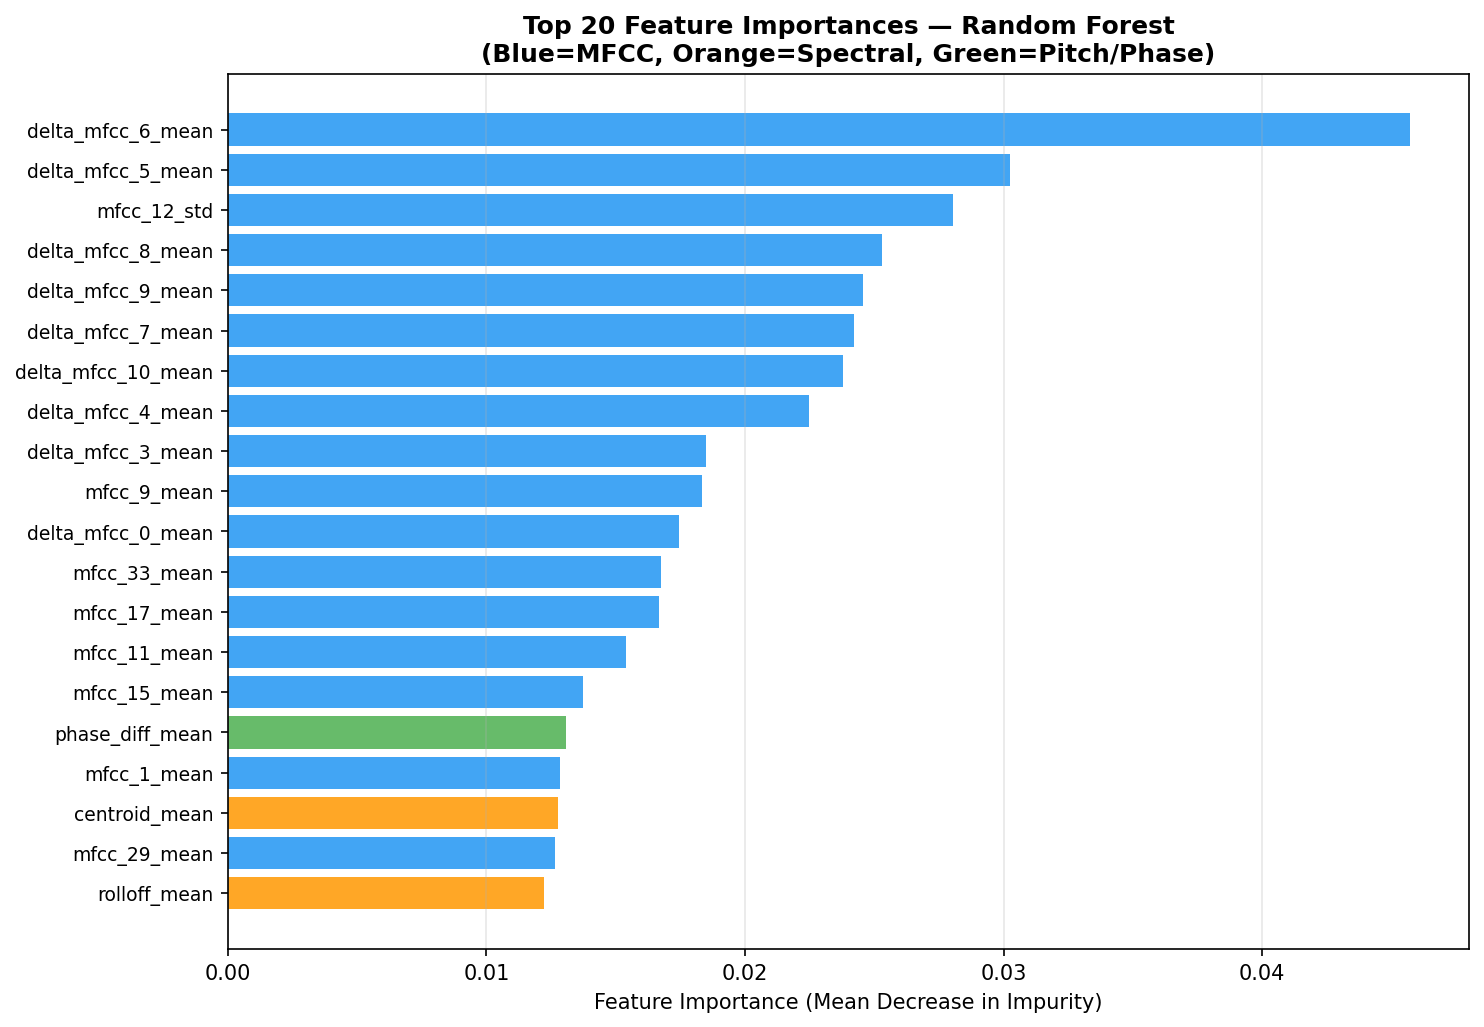
\includegraphics[width=0.85\textwidth]{feature_importance.png}
\caption{Top 20 feature importances from Random Forest (blue=MFCC, orange=spectral, green=pitch/phase). Delta-MFCC coefficients dominate, indicating temporal dynamics are the primary discriminative signal.}
\label{fig:features}
\end{figure}

\section{Deep Learning Results}

The CNN converged at epoch 22 (EER=0.0081, F1=0.9881, AUC=0.9993) --- comparable to SVM. The CNN-LSTM converged at epoch 21 and substantially outperformed the CNN: EER=0.0035, F1=0.9965, AUC=0.9996. This gap directly supports the hypothesis that temporal modelling via the LSTM captures prosodic artifacts that CNN global average pooling discards.

\begin{table}[H]
\centering
\caption{Deep learning model convergence summary}
\label{tab:convergence}
\renewcommand{\arraystretch}{1.25}
\begin{tabular}{L{2.5cm} C{2cm} C{2cm} C{2cm} C{3.5cm}}
\toprule
\tblhead{Model} & \tblhead{Parameters} & \tblhead{Best Epoch} & \tblhead{Val EER} & \tblhead{Training Time} \\
\midrule
\rowA CNN & 421,954 & 22 & 0.0154 & $\sim$55 min (RTX 3060) \\
\rowbest CNN-LSTM & \textbf{1,834,498} & \textbf{21} & \textbf{0.0092} & $\sim$60 min (RTX 3060) \\
\bottomrule
\end{tabular}
\end{table}

\begin{figure}[H]
\centering
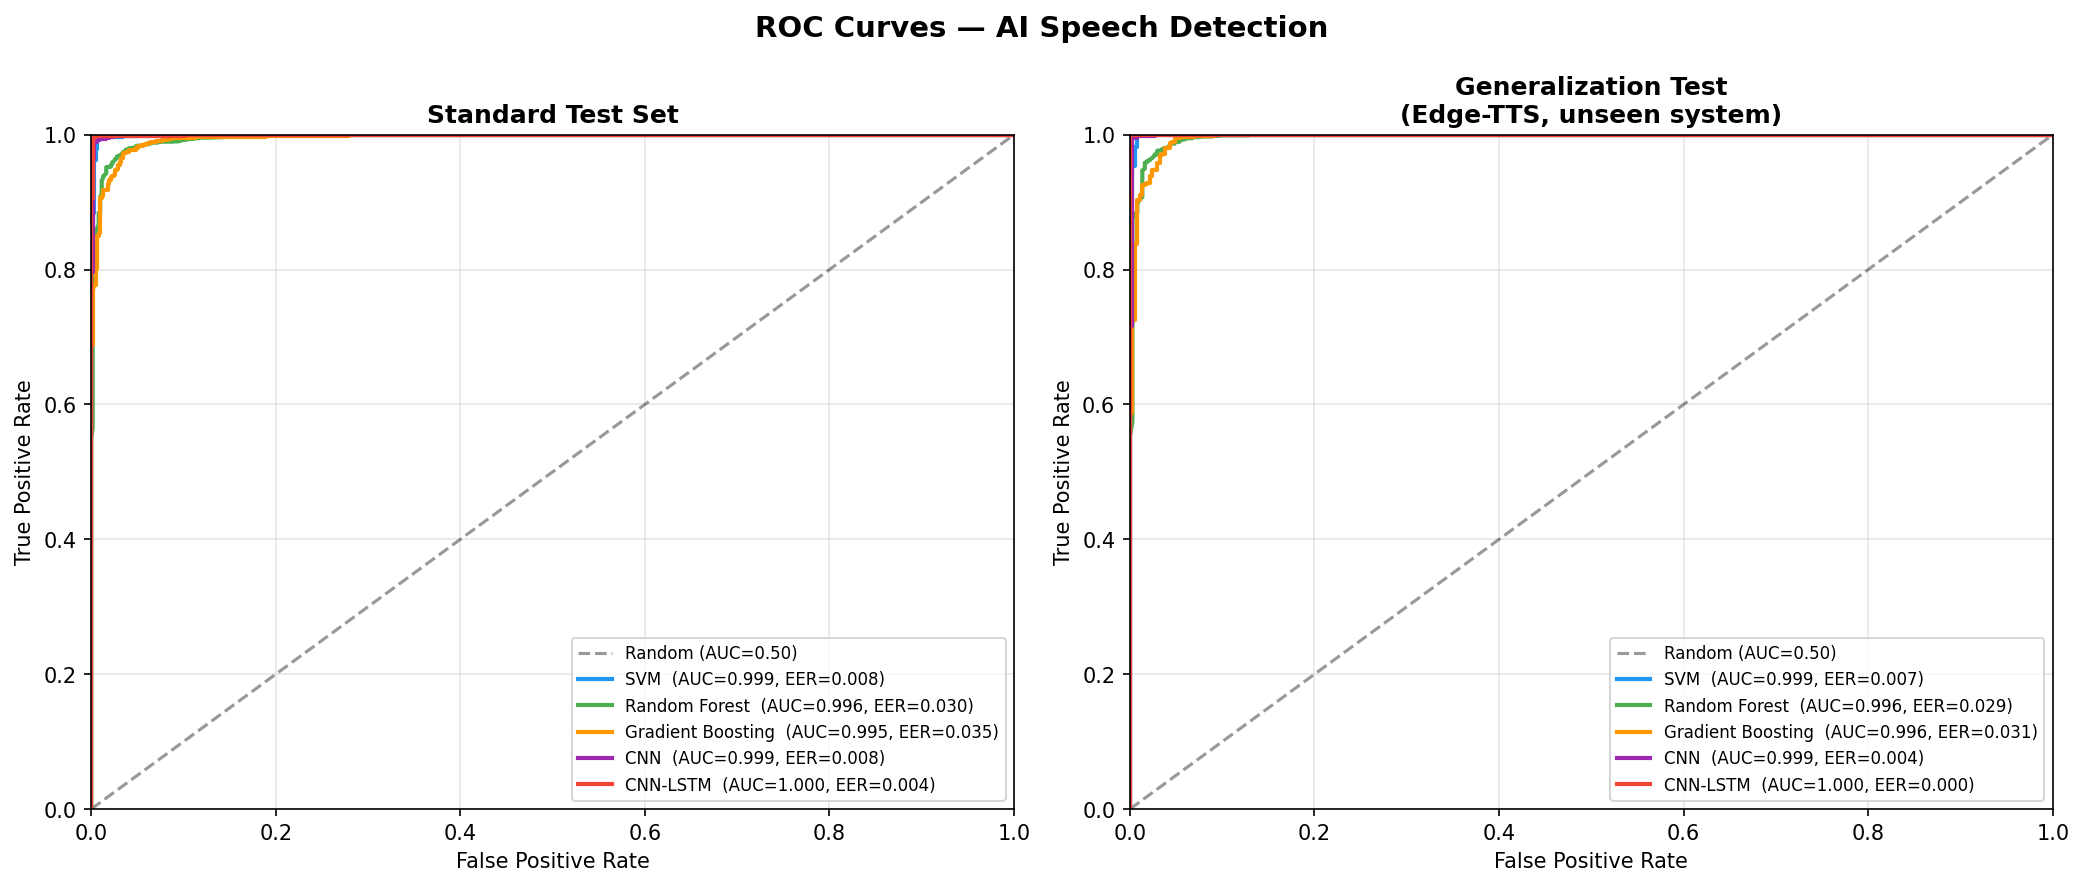
\includegraphics[width=\textwidth]{roc_curves.png}
\caption{ROC curves on the standard test set (left) and Edge-TTS generalization test (right). All models achieve high AUC; CNN-LSTM reaches AUC$=1.000$ on the generalization test.}
\label{fig:roc}
\end{figure}

\section{Generalization to Unseen TTS System}

All five models generalize well to the held-out Edge-TTS system, with every model achieving equal or lower EER on the generalization test than on the standard test (Table~\ref{tab:results}). The CNN-LSTM achieves EER$=0.0004$ (F1$=0.9978$, AUC$=1.000$) --- effectively perfect detection of a commercial TTS system absent from training. This counter-intuitive result (better performance on an unseen system) most likely reflects the consistency of Edge-TTS artifacts relative to the high diversity of ASVspoof 2019 systems. The practical implication is encouraging: models trained on diverse historical TTS systems generalize reliably to newer commercial systems.

\begin{figure}[H]
\centering
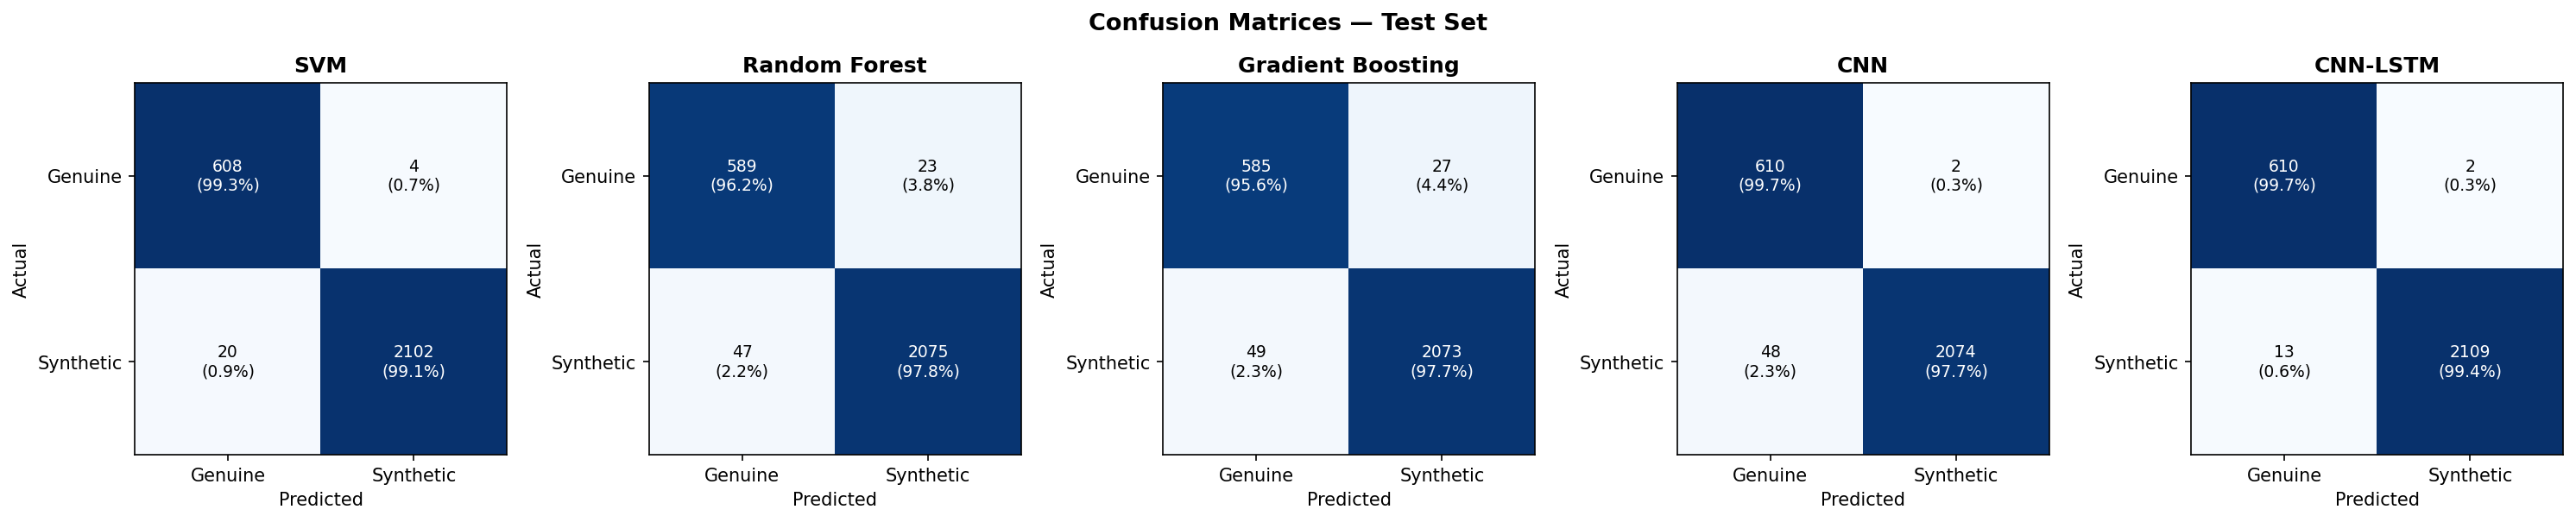
\includegraphics[width=\textwidth]{confusion_matrices.png}
\caption{Confusion matrices on the standard test set. CNN and CNN-LSTM achieve fewer than 3 false positives and under 50 false negatives per 2,734 test clips.}
\label{fig:cm}
\end{figure}

\section{Robustness Under Banking Telephony Conditions}

Figure~\ref{fig:degradation} shows robustness evaluation under noise and codec compression. Under clean conditions, SVM achieves near-zero EER. However, SVM degrades most rapidly with noise: EER$\approx 0.32$ at 20\,dB SNR, rising to $\approx 0.45$ at 5\,dB. Gradient Boosting shows the most noise-robust behaviour, flattening at $\approx 0.33$ below 15\,dB SNR. Under G.711 compression, all models degrade to EER 0.05--0.08 --- significant but manageable.

The key practical implication is that \textbf{noise is the more serious deployment threat than codec compression}. A production system should include noise reduction pre-processing or should be trained on noise-augmented data.

\begin{figure}[H]
\centering
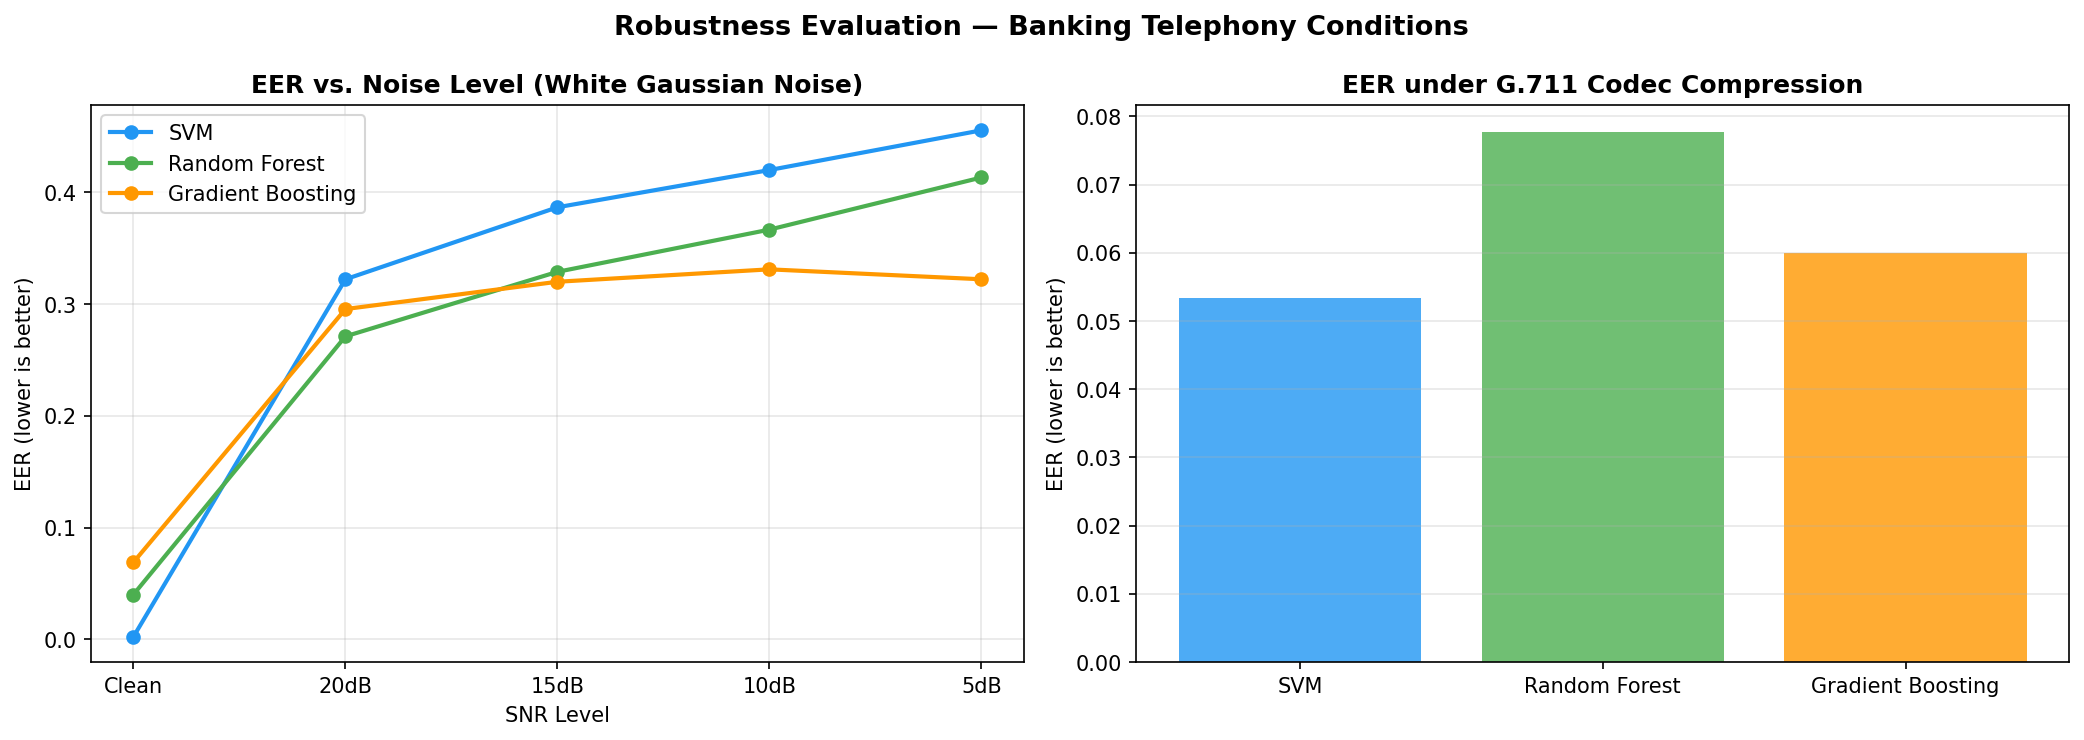
\includegraphics[width=\textwidth]{degradation_curves.png}
\caption{Robustness evaluation. Left: EER vs.\ SNR under white Gaussian noise. Right: EER under G.711 codec compression. Gradient Boosting is most noise-robust; all models degrade moderately under codec compression.}
\label{fig:degradation}
\end{figure}

\section{Consolidated Results and Comparison}

\begin{table}[H]
\centering
\caption{Full results across all models and evaluation conditions. EER: lower is better; F1, AUC, Acc: higher is better. $\dagger$ Generalization test = held-out Edge-TTS (unseen during training).}
\label{tab:results}
\renewcommand{\arraystretch}{1.3}
\begin{tabular}{L{3cm} L{3cm} C{1.4cm} C{1.4cm} C{1.4cm} C{1.4cm}}
\toprule
\tblhead{Model} & \tblhead{Evaluation Set} & \tblhead{EER $\downarrow$} & \tblhead{F1 $\uparrow$} & \tblhead{AUC $\uparrow$} & \tblhead{Acc $\uparrow$} \\
\midrule
\rowA SVM & Test & 0.0083 & 0.9943 & 0.9992 & 0.9912 \\
\rowA SVM & Gen.\ Test $\dagger$ & 0.0067 & 0.9969 & 0.9987 & 0.9953 \\
\rowB Random Forest & Test & 0.0305 & 0.9834 & 0.9956 & 0.9744 \\
\rowB Random Forest & Gen.\ Test $\dagger$ & 0.0293 & 0.9854 & 0.9964 & 0.9781 \\
\rowA Grad.\ Boosting & Test & 0.0346 & 0.9820 & 0.9949 & 0.9722 \\
\rowA Grad.\ Boosting & Gen.\ Test $\dagger$ & 0.0311 & 0.9868 & 0.9956 & 0.9801 \\
\rowdeep CNN & Test & 0.0081 & 0.9881 & 0.9993 & 0.9817 \\
\rowdeep CNN & Gen.\ Test $\dagger$ & 0.0036 & 0.9942 & 0.9991 & 0.9914 \\
\rowbest \textbf{CNN-LSTM} & \textbf{Test} & \textbf{0.0035} & \textbf{0.9965} & \textbf{0.9996} & \textbf{0.9945} \\
\rowbest \textbf{CNN-LSTM} & \textbf{Gen.\ Test $\dagger$} & \textbf{0.0004} & \textbf{0.9978} & \textbf{1.0000} & \textbf{0.9967} \\
\bottomrule
\end{tabular}
\end{table}

\begin{table}[H]
\centering
\caption{Indicative comparison with published anti-spoofing systems. Note: direct comparison is approximate --- evaluation conditions differ from benchmark studies.}
\label{tab:comparison}
\renewcommand{\arraystretch}{1.25}
\begin{tabular}{L{3.5cm} L{3cm} L{3cm} C{1.4cm} L{2.5cm}}
\toprule
\tblhead{Reference} & \tblhead{Dataset} & \tblhead{Method} & \tblhead{EER $\downarrow$} & \tblhead{Notes} \\
\midrule
\rowA \citet{todisco2019} & ASVspoof 2019 LA & CQCC + GMM & $\sim$0.10 & Official baseline \\
\rowB \citet{alzantot2019} & ASVspoof 2019 LA & ResNet spectrogram & $\sim$0.05 & CNN-based \\
\rowA \citet{wang2021aasist} & ASVspoof 2021 LA & AASIST (graph attn.) & $\sim$0.02 & SOTA at pub. \\
\rowB \citet{tak2022} & ASVspoof 2021 LA & RawBoost + ResNet & $\sim$0.015 & Data aug. focus \\
\rowbest This work --- SVM & Mixed, 10 TTS & MFCC + spectral & \textbf{0.0083} & Banking, 8\,kHz \\
\rowbest This work --- CNN-LSTM & Mixed, 10 TTS & Log-Mel CNN-LSTM & \textbf{0.0035} & Banking, 8\,kHz \\
\bottomrule
\end{tabular}
\end{table}

% ══════════════════════════════════════════════════════════════════════════════
% CHAPTER 5: CONCLUSION
% ══════════════════════════════════════════════════════════════════════════════
\chapter{Conclusion and Future Work}
\label{ch:conclusion}

\section{Summary of Findings}

This project developed and validated a complete pipeline for detecting AI-generated speech under banking telephony conditions, addressing all four research questions.

\textbf{RQ1 --- Reliability of detection:} All five models achieved EER below 0.035 and F1 above 0.98 on the standard test set. The CNN-LSTM achieved EER$=0.0035$. Detection is reliable across 10 TTS sources and 17,947 utterances under 8\,kHz telephony conditions.

\textbf{RQ2 --- Discriminative features:} Delta-MFCC coefficients emerged as the dominant discriminators, with spectral shape features and phase coherence as important secondary signals. TTS vocoders impose more regular and smoother temporal spectral dynamics than natural articulation.

\textbf{RQ3 --- Robustness under banking conditions:} Codec compression (G.711) degrades performance moderately (EER 0.05--0.08). Additive noise is more severe, degrading classical model EER to 0.32--0.45 at 5\,dB SNR. Gradient Boosting shows the best noise robustness. Noise reduction pre-processing or noise-aware training is needed for deployment in noisy call centre environments.

\textbf{RQ4 --- Deep vs.\ classical:} The CNN-LSTM (EER$=0.0035$) outperforms classical models, but the SVM with well-engineered features (EER$=0.0083$) is surprisingly competitive --- even outperforming the CNN alone. The incremental value of deep learning lies specifically in temporal modelling via the LSTM.

\section{Practical Implications for Banking Deployment}

A two-stage architecture is advisable: a lightweight SVM or Gradient Boosting for real-time screening (low latency) backed by a CNN-LSTM for borderline cases. Noise reduction should be applied upstream. The strong cross-system generalization results suggest that models trained on ASVspoof 2019 will be reasonably effective against commercial TTS systems in the near term, though continuous retraining as new TTS systems emerge is advisable.

\section{Limitations}

The genuine speech corpus (LibriSpeech) consists of clean audiobook readings rather than spontaneous conversational speech. The synthetic speech does not include the most recent diffusion-based models (e.g., Vall-E) which may present different artifact profiles. The robustness evaluation used white Gaussian noise rather than complex call centre noise. The dataset size is smaller than those used in top-performing published systems.

\section{Future Work}

Key extensions include: incorporating spontaneous speech corpora and diffusion-based TTS systems; fine-tuning wav2vec~2.0 or WavLM as a self-supervised encoder; noise-augmented training for improved robustness; online learning strategies to adapt to new TTS systems without full retraining; and end-to-end adversarial evaluation to assess security against attacks that exploit knowledge of the detection system.

% ══════════════════════════════════════════════════════════════════════════════
% BIBLIOGRAPHY
% ══════════════════════════════════════════════════════════════════════════════
\bibliographystyle{apalike}

\begin{thebibliography}{99}

\bibitem[Alzantot et al., 2019]{alzantot2019}
Alzantot, M., Wang, Z., and Srivastava, M.~B. (2019).
\newblock Deep Residual Neural Networks for Audio Spoofing Detection.
\newblock \textit{Proc.\ Interspeech 2019}, 1078--1082.

\bibitem[Baevski et al., 2020]{baevski2020}
Baevski, A., Zhou, Y., Mohamed, A., and Auli, M. (2020).
\newblock wav2vec 2.0: A Framework for Self-Supervised Learning of Speech Representations.
\newblock \textit{Advances in Neural Information Processing Systems (NeurIPS)}, 33.

\bibitem[Jia et al., 2018]{jia2018}
Jia, Y., Zhang, Y., Weiss, R.~J., et al. (2018).
\newblock Transfer Learning from Speaker Verification to Multispeaker Text-to-Speech Synthesis.
\newblock \textit{NeurIPS 2018}.

\bibitem[Kim et al., 2021]{kim2021vits}
Kim, J., Kong, J., and Son, J. (2021).
\newblock Conditional Variational Autoencoder with Adversarial Learning for End-to-End Text-to-Speech.
\newblock \textit{ICML 2021}.

\bibitem[Kinnunen et al., 2020]{kinnunen2020}
Kinnunen, T., Sahidullah, M., Falcone, M., et al. (2020).
\newblock t-DCF: a Detection Cost Function for the Tandem Assessment of Spoofing Countermeasures and Automatic Speaker Verification.
\newblock \textit{IEEE/ACM TASLP}.

\bibitem[McFee et al., 2015]{mcfee2015}
McFee, B., Raffel, C., Liang, D., et al. (2015).
\newblock librosa: Audio and Music Signal Analysis in Python.
\newblock \textit{Proceedings of the 14th Python in Science Conference}, 18--25.

\bibitem[Nautsch et al., 2021]{nautsch2021}
Nautsch, A., Wang, X., Evans, N., et al. (2021).
\newblock ASVspoof 2019: Spoofing Countermeasures for the Detection of Synthesized, Converted and Replayed Speech.
\newblock \textit{IEEE Transactions on Biometrics, Behavior, and Identity Science}.

\bibitem[Panayotov et al., 2015]{panayotov2015}
Panayotov, V., Chen, G., Povey, D., and Khudanpur, S. (2015).
\newblock Librispeech: An ASR Corpus Based on Public Domain Audio Books.
\newblock \textit{ICASSP 2015}.

\bibitem[Patel and Patil, 2015]{patel2015}
Patel, T.~B. and Patil, H.~A. (2015).
\newblock Combining Evidences from Mel Cepstral, Cochlear Filter Cepstral and Instantaneous Frequency Features for Detection of Natural vs.\ Spoofed Speech.
\newblock \textit{Interspeech 2015}, 2062--2066.

\bibitem[Ren et al., 2019]{ren2019fastspeech}
Ren, Y., Ruan, Y., Tan, X., et al. (2019).
\newblock FastSpeech: Fast, Robust and Controllable Text to Speech.
\newblock \textit{NeurIPS 2019}.

\bibitem[Sahidullah et al., 2015]{sahidullah2015}
Sahidullah, M., Kinnunen, T., and Hanilçi, C. (2015).
\newblock A Comparison of Features for Synthetic Speech Detection.
\newblock \textit{Interspeech 2015}, 2087--2091.

\bibitem[Shen et al., 2018]{shen2018}
Shen, J., Pang, R., Weiss, R.~J., et al. (2018).
\newblock Natural TTS Synthesis by Conditioning WaveNet on Mel Spectrogram Predictions.
\newblock \textit{ICASSP 2018}.

\bibitem[Tak et al., 2022]{tak2022}
Tak, H., Patino, J., Todisco, M., et al. (2022).
\newblock End-to-End Spectro-Temporal Graph Attention Networks for Speaker Verification Anti-Spoofing and Speech Deepfake Detection.
\newblock \textit{ASVspoof 2021 Workshop}.

\bibitem[Todisco et al., 2019]{todisco2019}
Todisco, M., Wang, X., Vestman, V., et al. (2019).
\newblock ASVspoof 2019: Future Horizons in Spoofed and Fake Speech Detection.
\newblock \textit{Interspeech 2019}.

\bibitem[van den Oord et al., 2016]{vandendoord2016}
van den Oord, A., Dieleman, S., Zen, H., et al. (2016).
\newblock WaveNet: A Generative Model for Raw Audio.
\newblock \textit{arXiv:1609.03499}.

\bibitem[Wang et al., 2017]{wang2017tacotron}
Wang, Y., Skerry-Ryan, R.~J., Stanton, D., et al. (2017).
\newblock Tacotron: Towards End-to-End Speech Synthesis.
\newblock \textit{Interspeech 2017}.

\bibitem[Wang et al., 2021]{wang2021aasist}
Wang, T., Yi, J., Fu, R., et al. (2021).
\newblock AASIST: Audio Anti-Spoofing using Integrated Spectro-Temporal Graph Attention Networks.
\newblock \textit{ICASSP 2022}.

\bibitem[Yi et al., 2022]{yi2022}
Yi, J., Fu, R., Tao, J., et al. (2022).
\newblock Add 2022: the First Audio Deep Synthesis Detection Challenge.
\newblock \textit{ICASSP 2022}.

\end{thebibliography}

\end{document}